%-----------------------------------------------------------------------------------------------------------------------------------------------%
%	The MIT License (MIT)
%
%	Copyright (c) 2021 Lucas GRELAUD
%
%	Permission is hereby granted, free of charge, to any person obtaining a copy
%	of this software and associated documentation files (the "Software"), to deal
%	in the Software without restriction, including without limitation the rights
%	to use, copy, modify, merge, publish, distribute, sublicense, and/or sell
%	copies of the Software, and to permit persons to whom the Software is
%	furnished to do so, subject to the following conditions:
%	
%	THE SOFTWARE IS PROVIDED "AS IS", WITHOUT WARRANTY OF ANY KIND, EXPRESS OR
%	IMPLIED, INCLUDING BUT NOT LIMITED TO THE WARRANTIES OF MERCHANTABILITY,
%	FITNESS FOR A PARTICULAR PURPOSE AND NONINFRINGEMENT. IN NO EVENT SHALL THE
%	AUTHORS OR COPYRIGHT HOLDERS BE LIABLE FOR ANY CLAIM, DAMAGES OR OTHER
%	LIABILITY, WHETHER IN AN ACTION OF CONTRACT, TORT OR OTHERWISE, ARISING FROM,
%	OUT OF OR IN CONNECTION WITH THE SOFTWARE OR THE USE OR OTHER DEALINGS IN
%	THE SOFTWARE.
%	
%
%-----------------------------------------------------------------------------------------------------------------------------------------------%


%============================================================================%
%
%	DOCUMENT DEFINITION
%
%============================================================================%

%we use article class because we want to fully customize the page and dont use a cv template
\documentclass[10pt,A4]{article}	


%----------------------------------------------------------------------------------------
%	ENCODING
%----------------------------------------------------------------------------------------

%we use utf8 since we want to build from any machine
\usepackage[utf8]{inputenc}		

%----------------------------------------------------------------------------------------
%	LOGIC
%----------------------------------------------------------------------------------------

% provides \isempty test
\usepackage{xifthen}

%----------------------------------------------------------------------------------------
%	FONT
%----------------------------------------------------------------------------------------

% some tex-live fonts - choose your own

\usepackage[defaultsans]{droidsans}
%\usepackage[default]{comfortaa}
%\usepackage{cmbright}
%\usepackage[default]{raleway}
%\usepackage{fetamont}
%\usepackage[default]{gillius}
%\usepackage[light,math]{iwona}
%\usepackage[thin]{roboto} 

% set font default
\renewcommand*\familydefault{\sfdefault} 	
\usepackage[T1]{fontenc}

% more font size definitions
\usepackage{moresize}		


%----------------------------------------------------------------------------------------
%	PAGE LAYOUT  DEFINITIONS
%----------------------------------------------------------------------------------------

%debug page outer frames
%\usepackage{showframe}			


%define page styles using geometry
\usepackage[a4paper]{geometry}		

% for example, change the margins to 2 inches all round
\geometry{top=1.75cm, bottom=-.6cm, left=1.5cm, right=1.5cm} 	

%use customized header
\usepackage{fancyhdr}				
\pagestyle{fancy}

%less space between header and content
\setlength{\headheight}{-5pt}		


%customize entries left, center and right
\lhead{}
\chead{ \small{Lucas GRELAUD $\cdot$ Ingénieur en Sécurité des Systèmes Embarqués $\cdot$  Chatou, FRANCE 

\textcolor{sectcol}{\textbf{lucas.grelaud@outlook.fr}}  $\cdot$ +33 6 33 90 50 61}}
\rhead{}


%indentation is zero
\setlength{\parindent}{0mm}

%----------------------------------------------------------------------------------------
%	TABLE /ARRAY/LIST DEFINITIONS
%---------------------------------------------------------------------------------------- 

%for layouting tables
\usepackage{multicol}			
\usepackage{multirow}

%extended aligning of tabular cells
\usepackage{array}

\newcolumntype{x}[1]{%
>{\raggedleft\hspace{0pt}}p{#1}}%

\usepackage{enumitem}


%----------------------------------------------------------------------------------------
%	GRAPHICS DEFINITIONS
%---------------------------------------------------------------------------------------- 

%for header image
\usepackage{graphicx}

%for floating figures
\usepackage{wrapfig}
\usepackage{float}
%\floatstyle{boxed} 
%\restylefloat{figure}

%for drawing graphics		
\usepackage{tikz}				
\usetikzlibrary{shapes, backgrounds,mindmap, trees}


%----------------------------------------------------------------------------------------
%	Color DEFINITIONS
%---------------------------------------------------------------------------------------- 

\usepackage{color}

%accent color
\definecolor{bgcol}{RGB}{89,98,117}

%dark background color
\definecolor{sectcol}{RGB}{226,84,64}

%light background / accent color
\definecolor{softcol}{RGB}{225,225,225}


%============================================================================%
%
%
%	DEFINITIONS
%
%
%============================================================================%

%----------------------------------------------------------------------------------------
% 	HEADER
%----------------------------------------------------------------------------------------

% remove top header line
\renewcommand{\headrulewidth}{0pt} 

%remove botttom header line
\renewcommand{\footrulewidth}{0pt}	  	

%remove pagenum
\renewcommand{\thepage}{}	

%remove section num		
\renewcommand{\thesection}{}			

%----------------------------------------------------------------------------------------
% 	ARROW GRAPHICS in Tikz
%----------------------------------------------------------------------------------------

% a six pointed arrow poiting to the left
\newcommand{\tzlarrow}{(0,0) -- (0.2,0) -- (0.3,0.2) -- (0.2,0.4) -- (0,0.4) -- (0.1,0.2) -- cycle;}	

% include the left arrow into a tikz picture
% param1: fill color
%
\newcommand{\larrow}[1]
{\begin{tikzpicture}[scale=0.58]
	 \filldraw[fill=#1!100,draw=#1!100!black]  \tzlarrow
 \end{tikzpicture}
}

% a six pointed arrow poiting to the right
\newcommand{\tzrarrow}{ (0,0.2) -- (0.1,0) -- (0.3,0) -- (0.2,0.2) -- (0.3,0.4) -- (0.1,0.4) -- cycle;}

% include the right arrow into a tikz picture
% param1: fill color
%
\newcommand{\rarrow}
{
\begin{tikzpicture}[scale=0.7]
	\filldraw[fill=sectcol!100,draw=sectcol!100!black] \tzrarrow
 \end{tikzpicture}
}



%----------------------------------------------------------------------------------------
%	custom sections
%----------------------------------------------------------------------------------------

% create a coloured box with arrow and title as cv section headline
% param 1: section title
%
\newcommand{\cvsection}[1]
{
\colorbox{bgcol}{\makebox[1\linewidth][l]{
	\larrow{sectcol} \hspace{-8pt} \larrow{sectcol} \hspace{-8pt} \larrow{sectcol} \textcolor{white}{\textbf{#1}}\hspace{4pt}
}}\\
}

%create a coloured arrow with title as cv meta section section
% param 1: meta section title
%
\newcommand{\metasection}[2]{
	\begin{tabular*}{1\linewidth}{p{0.21\linewidth} p{0.75\linewidth}}
		\larrow{bgcol}\normalsize{\textbf{\textcolor{sectcol}{#1}}}&#2\\
	\end{tabular*}
}

%----------------------------------------------------------------------------------------
%	 CV EVENT
%----------------------------------------------------------------------------------------

% creates a stretched box as cv entry headline followed by two paragraphs about 
% the work you did
% param 1:	event time i.e. 2014 or 2011-2014 etc.
% param 2:	event name (what did you do?)
% param 3:	institution (where did you work / study)
% param 4:	what was your position
% param 5:	some words about your contributions
%
\newcommand{\cvevent}[5] {
\begin{flushleft}
\textcolor{sectcol}{#1 - #3}\\
\textbf{#2}\\[-7pt]
\textcolor{softcol}{\hrule}
\vspace{\spread}
\begin{tabular*}{1\linewidth}{p{0.001\linewidth} p{0.9\linewidth}}
	\larrow{bgcol} & #4 \\[2pt]
	\larrow{bgcol} & #5 \\[\spread]
\end{tabular*}
\end{flushleft}

%\textcolor{softcol}{\hrule}
}

% creates a stretched box as 
\newcommand{\cveventmeta}[2] {
	\mbox{\mystrut \hspace{87pt}\textit{#1}}\\
	#2
}

%----------------------------------------------------------------------------------------
% CUSTOM STRUT FOR EMPTY BOXES
%----------------------------------------- -----------------------------------------------
\newcommand{\mystrut}{\rule[-.3\baselineskip]{0pt}{\baselineskip}}

%----------------------------------------------------------------------------------------
% CUSTOM LOREM IPSUM
%----------------------------------------------------------------------------------------
\newcommand{\lorem}
{Lorem ipsum dolor sit amet, consectetur adipiscing elit. Donec a diam lectus.}

%----------------------------------------------------------------------------------------
% SPREAD
%----------------------------------------------------------------------------------------
\newcommand{\spread}{7pt}

%============================================================================%
%
%
%
%	DOCUMENT CONTENT
%
%
%
%============================================================================%
\begin{document}


%use our custom fancy header definitions
\pagestyle{fancy}



\begin{minipage}[t]{0.485\textwidth}

\vspace{\spread}

%---------------------------------------------------------------------------------------
%	TITLE HEADLINE
%----------------------------------------------------------------------------------------

\hspace{-0.25\linewidth}\colorbox{bgcol}{\makebox[1.25\linewidth][c]{\HUGE{\textcolor{white}{\textsc{Lucas}}} \textcolor{sectcol}{\rule[-1mm]{1mm}{0.9cm}} \HUGE{\textcolor{white}{\textsc{GRELAUD}} } }}

%----------------------------------------------------------------------------------------
%	HEADER IMAGE
%----------------------------------------------------------------------------------------
\hspace{-0.25\linewidth}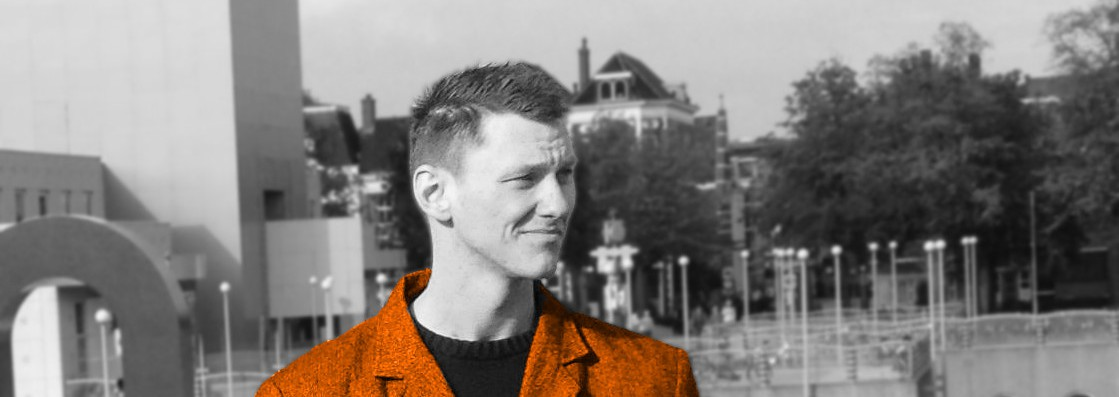
\includegraphics[width=1.2725\linewidth]{myfoto.jpg} %use full size

%---------------------------------------------------------------------------------------
%	QR CODE (optional)
%----------------------------------------------------------------------------------------
\vspace{-100pt}
\hspace{0.59\linewidth}

\includegraphics[width=88pt]{qrcode}
\normalsize


\vspace{20pt}

\end{minipage} 
\hfill
\begin{minipage}[t]{0.485\textwidth}
%---------------------------------------------------------------------------------------
%	SUMMARY (optional)
%----------------------------------------------------------------------------------------
\vspace{\spread}

\cvsection{À Propos}\\
Bientôt diplômé du titre d'Ingénieur en Système Embarqué, je prépare actuellement mon mémoire de fin d'étude sur la sécurisation de l'infrastructure DevOps du groupe JCDecaux.\\

Cette formation un peu atypique, académique en Système Embarqué et professionnel en Sécurité Informatique, me permets d'avoir une meilleure vision des problématiques liés à la sécurisation de systèmes industriel et tout particulièrement des IoT.\\[-2pt]
\textcolor{softcol}{\hrule}

\end{minipage}

\begin{minipage}[t]{0.485\textwidth}

\vspace{\spread}

%---------------------------------------------------------------------------------------
%	META SECTION
%----------------------------------------------------------------------------------------
\metasection{Activité:}{Ingénieur en sécurité Informatique, JCDecaux SA, Apprenti}
\metasection{Secteurs:}{Système Embarqué, Sécurité Informatique, Ingénierie} 
\end{minipage}
\hfill
\begin{minipage}[t]{0.485\textwidth}

\vspace{5pt}

\metasection{Tech:}{C/C++, Python, QT5, VHDL, Burp, Wireshark, InsighVM, Suricata, Wazuh, ...}
\metasection{Intérêts:}{IoT, HomeLab, Aérospatial amateur, engagement associatif}
\end{minipage}


\begin{minipage}[t]{0.485\textwidth}

\vspace{\spread}

%---------------------------------------------------------------------------------------
%	EDUCATION SECTION
%--------------------------------------------------------------------------------------

\cvsection{Formation}

\cvevent{2018 - 2021}{Cycle Ingénieur, spécialisation Système Embarqué}
	{ESIEA}
	{Mémoire : <Titre mémoire>}
	{Architecture de systèmes Embarqué et systèmes communiquant}
Activité : Gestion logistique de l'association Air-ESIEA \& Membre de l'équipe de conception / réalisation du FabLab de l'ESIEA Paris

%\textcolor{softcol}{\hrule}

%
\cvevent{2018}{Semestre international}
	{Université du Québec  à Chicoutimi}
	{Modules de Développement Web Avancé, Android, Sécurité Informatique}
	{Stage en laboratoire de recherche}
Activité : Membre du Club de Robotique de l'UQAC
%\textcolor{softcol}{\hrule}

%
\cvevent{2016 - 2018}{DUT Informatique}
	{IUT de Montreuil, Université Paris VIII}
	{Architecture et Développement de logiciel}
	{Administration systèmes et réseau}
%\textcolor{softcol}{\hrule}

%
\cvevent{2013 - 2016}{Baccalauréat Technologique, STI2D option Énergie et Environnement}
	{Lycée Léonard de Vinci, Saint-Germain-en-Laye}
	{Électrotechnique et Automatique industrielle}
	{Optimisation énergétique de systèmes}
%\textcolor{softcol}{\hrule}


\end{minipage}
\hfill
\begin{minipage}[t]{0.485\textwidth}

\vspace{\spread}

%---------------------------------------------------------------------------------------
%	EXPERIENCE
%----------------------------------------------------------------------------------------
\cvsection{Experience}

%
\cvevent{2018 - 2021}{Ingénieur Sécurité Informatique, apprentissage}
	{JCDecaux SA}
	{Qualification sécurité des applications du groupe etd'équipements en vue de déploiement}
	{PoC et/ou déploiement de solutions de sécurité (Rapid7 InsighVM, Wazuh, Swordphish, ...)}

%
\cvevent{2018, 3 mois}{Développeur logiciel}
	{Laboratoire d'Intelligence Ambiante pour la Reconnaissance d'Activités}
	{Analyse et visualisation de données}
	{Création d'interfaces de labellisation  de données pour la création de DataSets}

%
\cvevent{2017 - 2018}{Ambassadeur de marque}
	{Conrad Electronic Group}
	{Promotion des produits de l'enseigne}
	{Création de tutoriels et guide d'utilisation de produit / technologies vendu par Conrad}


\end{minipage}

%-------------------------------------------------------------------------------------------------
%	ARTIFICIAL FOOTER (fancy footer cannot exceed linewidth) 
%--------------------------------------------------------------------------------------------------

\null
\vspace*{\fill}
\hspace{-0.25\linewidth}\colorbox{bgcol}{\makebox[1.5\linewidth][c]{\mystrut  \textcolor{white}{www.grelaud.eu} $\cdot$ \textcolor{white}{github.com/lucasgrelaud}}}




%============================================================================%
%
%
%
%	DOCUMENT END
%
%
%
%============================================================================%
\end{document}
